%% ===========================================================================
\appendix

\section{Collection queries}
\label{app:queries}

We collected submissions by keyword search within each collected community (\S\ref{sec:data-collection}). Table~\ref{tab:queries} lists the 39 queries recorded in our collection export, grouped by topic, with the number of
submissions each matched in each collection pass. We ran the baseline pass over 1 January 2019 to 30 December 2025 in every collected community, the crisis-window pass over five windows between 2019 and 2021 in nine communities,
and a third pass over 7 to 10 May 2025 in six communities. A submission can match several queries, so a column sums to more than the submissions in it; the last rows give the distinct submissions and the number of queries in each pass.

\begin{table}[htbp]
\centering
\caption{Collection queries, grouped by topic, and the submissions each matched in
each collection pass.}
\label{tab:queries}
\footnotesize
\setlength{\tabcolsep}{4pt}
\begin{tabular}{@{}lrrrr@{}}
\toprule
query & baseline & crisis windows & 7--10 May 2025 & total \\
\midrule
\multicolumn{5}{@{}l}{\itshape India and Pakistan named together} \\
India Pakistan & 16,509 & 3,507 & 1,639 & 21,655 \\
Modi Pakistan & 1,534 & 0 & 0 & 1,534 \\
Imran Khan India & 873 & 0 & 0 & 873 \\
India-{}Pakistan & 604 & 0 & 0 & 604 \\
Indo-{}Pak & 391 & 0 & 0 & 391 \\
Indo Pakistan & 334 & 0 & 0 & 334 \\
Bharat Pakistan & 259 & 0 & 0 & 259 \\
Sharif India & 188 & 0 & 0 & 188 \\
bilateral talks & 183 & 0 & 0 & 183 \\
Hindustan Pakistan & 139 & 0 & 0 & 139 \\
\addlinespace
\multicolumn{5}{@{}l}{\itshape Kashmir} \\
Kashmir & 0 & 4,246 & 0 & 4,246 \\
Jammu Kashmir & 3,680 & 0 & 0 & 3,680 \\
Article 370 & 1,954 & 647 & 0 & 2,601 \\
Kashmir India Pakistan & 1,978 & 0 & 0 & 1,978 \\
Kashmir conflict & 471 & 0 & 0 & 471 \\
\addlinespace
\multicolumn{5}{@{}l}{\itshape Attacks} \\
Pulwama & 2,546 & 971 & 0 & 3,517 \\
Pahalgam & 72 & 0 & 231 & 303 \\
Jaish & 0 & 181 & 0 & 181 \\
CRPF attack & 0 & 95 & 0 & 95 \\
\addlinespace
\multicolumn{5}{@{}l}{\itshape Military action} \\
Balakot & 1,100 & 230 & 0 & 1,330 \\
war & 0 & 0 & 1,092 & 1,092 \\
surgical strike & 698 & 129 & 13 & 840 \\
cross-{}border & 511 & 0 & 0 & 511 \\
IAF Pakistan & 450 & 0 & 0 & 450 \\
Operation Sindoor & 0 & 0 & 396 & 396 \\
airstrike & 0 & 133 & 107 & 240 \\
airstrike India & 155 & 0 & 0 & 155 \\
PAF India & 88 & 0 & 0 & 88 \\
military strike & 0 & 0 & 83 & 83 \\
\addlinespace
\multicolumn{5}{@{}l}{\itshape Border and ceasefire} \\
LOC & 1,420 & 26 & 85 & 1,531 \\
Line of Control & 1,223 & 0 & 0 & 1,223 \\
ceasefire & 0 & 67 & 946 & 1,013 \\
ceasefire violation & 371 & 0 & 0 & 371 \\
DGMO & 6 & 0 & 0 & 6 \\
\addlinespace
\multicolumn{5}{@{}l}{\itshape Nuclear weapons} \\
nuclear war & 5,010 & 0 & 0 & 5,010 \\
nuclear India & 1,815 & 0 & 0 & 1,815 \\
nuclear Pakistan & 1,082 & 0 & 0 & 1,082 \\
nuclear threat & 1,002 & 0 & 0 & 1,002 \\
nuclear & 0 & 0 & 108 & 108 \\
\midrule
submissions matching any query & 36,767 & 9,145 & 3,582 & 49,494 \\
queries used in the pass & 30 & 11 & 10 & 39 \\
\bottomrule
\end{tabular}
\vspace{2pt}
{\footnotesize Counts are submissions in the collection export, before
deduplication. The grouping is ours.\par}
\end{table}

\section{Codebook}
\label{app:codebook}

Our coders labelled with a written codebook (version~3, March 2026), and they made the targeting decision with a separate set of rules. Below we condense both to the layers this paper reports. For each layer we give the unit coded, the labels with their definitions, and the rule that decides between labels. The model prompts in Appendix~\ref{app:prompts} draw on the same definitions and rules.

\begin{enumerate}
\item \textbf{Relevance} (one label per submission).
\begin{itemize}
\item \textit{Relevant}: \authorinput{the definition given to the gate and to the
two coders}
\item \textit{Irrelevant}: \authorinput{the definition, including whether cricket
and the Indus Waters Treaty count as relevant}
\end{itemize}

\item \textbf{Content type} (one label per comment).
\begin{itemize}
\item \textit{Factual claim}: asserts a proposition about the real world that can
in principle be checked against evidence, and does nothing else. The test is
whether the sentence could appear as written in a news-wire report.
\item \textit{Opinion or commentary}: expresses a belief, evaluation,
interpretation or moral judgement, including a prediction. A comment that cites
facts in order to argue, evaluate or persuade is an opinion.
\item \textit{Question}: has an interrogative structure and seeks information,
including rhetorical questions.
\item \textit{Satire or humour}: shows explicit satire markers (such as
\texttt{/s}), meme-like exaggeration, irony or parody, with no serious intent to
assert a fact.
\end{itemize}
Coders ask three questions in order. Is the comment primarily a question? Then it
is a \textit{question}. Is its primary intent satire, humour or parody? Then it is
\textit{satire or humour}. Does it assert a verifiable claim with no evaluative or
argumentative framing at all? Then it is a \textit{factual claim}; otherwise it is
\textit{opinion or commentary}. When facts and evaluation occur together, the
comment is an opinion: if stripping the evaluative language removes the
comment's point, it was an opinion. When in doubt between a factual claim and an
opinion, coders choose opinion. In our analysis we collapse this layer to opinion
against the other three labels (\S\ref{sec:data-constructs}).

\item \textbf{Narrative frame} (one dominant frame per comment).
\begin{itemize}
\item \textit{Security and military}: the conflict as armed confrontation, military
action, retaliation, deterrence or a threat to national security. Includes
terrorism, nuclear escalation, and a ceasefire framed as the end of military
action.
\item \textit{Humanitarian}: the conflict through civilian suffering, human-rights
violations, displacement or responsibility toward non-combatants.
\item \textit{Political}: the conflict through government decisions, parties,
leaders, constitutional change, elections or regime responsibility, including
diplomacy framed as a political process.
\item \textit{Economic}: the conflict through economic harm or benefit, sanctions,
trade, development or the cost of war.
\item \textit{Historical grievance}: the conflict as rooted in past injustice, with
history as the main explanation, for example Partition and 1947.
\item \textit{Religious or cultural}: the conflict as a clash of religious
identities or cultural values, with religion or culture as the central
explanation.
\end{itemize}
Coders choose the frame that structures the comment's explanation of the
conflict, not the one mentioned most often or last, by asking why, according to
the comment, the conflict is happening. A comment that mentions military
operations but centres on civilian casualties is \textit{humanitarian}. Explicit
religious identity markers (such as Islam, Muslim, Hindu, jihad or Hindutva) used
to frame the conflict route to \textit{religious or cultural}, even when political
actors are named. If a comment is too general to frame on its own, coders use the
title of its submission as the anchor. An earlier version of the codebook had
eight frames; after the pilot round we merged nuclear threat into \textit{security
and military} and divided peace and diplomacy between \textit{political} and
\textit{security and military}.

\item \textbf{Sentiment} (one label per comment).
\begin{itemize}
\item \textit{Positive}: support, approval, hope, optimism, relief or another
favourable evaluation.
\item \textit{Negative}: criticism, disapproval, anger, frustration, pessimism,
concern or condemnation.
\item \textit{Neutral}: factual reporting, a balanced presentation of several
perspectives, or no clear evaluative position.
\end{itemize}
Coders code sarcasm by its intended meaning, so ``Oh great, another surgical
strike'' is \textit{negative}. When sentiments mix, they assign the dominant one,
and a truly balanced comment is \textit{neutral}.

\item \textbf{Stance toward India} and \textbf{stance toward Pakistan} (one label
per comment on each axis).
\begin{itemize}
\item \textit{Pro}: support, defence, justification or sympathy toward the country,
its government, its military or its people, including praise and positive
framing.
\item \textit{Anti}: criticism, condemnation, blame or hostility toward the
country, its government, its military or its people, including negative framing
and accusations.
\item \textit{Neutral}: the comment mentions the country without a clear stance,
reports facts, is genuinely balanced, or gives too little to infer a stance.
\end{itemize}
Coders label the two axes independently: supporting India does not imply opposing
Pakistan, and all nine combinations are valid. Stance can be implicit. Praising
``the Indian military's restraint'' is \textit{pro} India even if the comment never
names India, and criticising ``ISI interference'' is \textit{anti} Pakistan.

\item \textbf{Toxicity check} (one label per comment, for the 200 comments sampled
on both sides of Perspective's threshold).
\begin{itemize}
\item \textit{Offensive, targeted}: inappropriate language, insults or threats
directed at a specific individual or group.
\item \textit{Offensive, untargeted}: profanity, vulgar language or other offensive
content without a clear target.
\item \textit{Not offensive}: none of the above.
\end{itemize}
In the corpus, the decision between toxic and not toxic is Perspective's threshold
(\S\ref{sec:data-constructs}). To score that threshold against the coders, we
count both offensive labels as toxic.

\item \textbf{Target} (one label per comment, for comments Perspective scores as
toxic). The question is whether the offensive language attacks an identifiable
person, group, nation or religion. Coders apply the tests below in order and stop
at the first that holds.
\begin{itemize}
\item \textit{Named entity}: the insult names, or is aimed at, a person, country,
political party or organisation (``Modi is a fascist dictator'', ``ISI funds
terrorism''). Targeted.
\item \textit{Pronoun}: \textit{you} or \textit{your} in the scope of an insult
attacks the person being addressed, and \textit{they} or \textit{them} referring
to a group in the scope of an insult attacks that group. Targeted.
\item \textit{Group noun}: a demonym, a religious, caste or ethnic term, or a
political label (such as \textit{bhakt} or \textit{sanghi}) in the scope of an
insult. Targeted.
\item \textit{Coded slur}: a coded slur, deliberate misspelling or dehumanising
metaphor (vermin, disease) for an identifiable group, even when the tone is
informal or joking. Targeted.
\item \textit{Sarcasm}: sarcasm or irony that attacks an identifiable group despite
positive surface words. Targeted.
\item \textit{Intensifier}: profanity that intensifies or vents about a situation,
an event or an abstract idea rather than an entity. Untargeted. Profanity aimed
at a group or an institution is targeted.
\item \textit{Unclear reference}: if \textit{they}, \textit{them} or \textit{these
people} can be resolved to an identifiable group from the submission title or
earlier sentences, targeted; otherwise untargeted.
\end{itemize}
A comment that quotes someone else's offensive speech is labelled by the
commenter's own position: quoting it to criticise it is untargeted, and endorsing
the quoted attack is targeted. When the target cannot be determined, coders
choose untargeted.
\end{enumerate}

\section{Labeller benchmark}
\label{app:benchmark}

Table~\ref{tab:benchmark} scores each system we tested against the adjudicated
reference for its layer and lists our two coders' agreement beside it for
comparison. It uses the full annotation samples, which we drew before we fixed the
ten communities, so its coder values differ slightly from
Table~\ref{tab:reliability}; because the samples differ by layer, we compare
systems only within a layer. The table leaves out systems that failed rather than
underperformed, such as the three stance classifiers built on natural-language
inference, which put every comment in one class.

% \begin{table}[H]
% \centering
% \caption{Labellers compared against each construct's gold standard before any
% was adopted.}
% \label{tab:benchmark}
% \begin{tabular}{llrr}
% \toprule
% Construct & Labeller & $\kappa$ & $n$ \\
% \midrule
% \multirow{2}{*}{content type}
%   & trained coder pair                         & 0.612 & 250 \\
%   & commercial LLM, zero-shot                  & 0.599 & 250 \\
% \midrule
% \multirow{2}{*}{narrative frame}
%   & trained coder pair                         & 0.665 & 250 \\
%   & commercial LLM, zero-shot                  & 0.688 & 250 \\
% \midrule
% \multirow{5}{*}{sentiment}
%   & trained coder pair                         & 0.549 & 250 \\
%   & lexicon and rules                          & 0.157 & 250 \\
%   & encoder, pre-trained                       & 0.374 & 250 \\
%   & open-weight LLM, self-consistency          & 0.526 & 250 \\
%   & open-weight LLM, parameter-efficient tuning & 0.566 & 250 \\
% \midrule
% \multirow{2}{*}{stance toward India}
%   & trained coder pair                         & 0.521 & 250 \\
%   & open-weight LLM, self-consistency          & 0.407 & 250 \\
% \midrule
% \multirow{2}{*}{stance toward Pakistan}
%   & trained coder pair                         & 0.557 & 250 \\
%   & open-weight LLM, zero-shot                 & 0.455 & 250 \\
% \midrule
% \multirow{6}{*}{target type}
%   & trained coder pair                         & 0.682 & 500 \\
%   & deployed commercial classifier             & 0.228 & 500 \\
%   & encoder, pre-trained                       & 0.377 & 500 \\
%   & open-weight LLM, zero-shot                 & 0.416 & 500 \\
%   & open-weight LLM, parameter-efficient tuning & 0.480 & 500 \\
%   & encoder, fine-tuned                        & 0.487 & 500 \\
% \bottomrule
% \end{tabular}
% \end{table}


\begin{table}[htbp]
\centering
\caption{Agreement of each labeller we tested with the adjudicated human reference
for each layer, beside the agreement between our two coders.}
\label{tab:benchmark}
\small
\setlength{\tabcolsep}{3pt}
\begin{tabularx}{\linewidth}{@{}>{\raggedright\arraybackslash}p{1.55cm}l>{\raggedright\arraybackslash}Xrr@{}}
\toprule
layer & system & approach & $\kappa$ & $n$ \\
\midrule
content type & two coders &  & 0.612 & 250 \\
 & gpt-5.2 & zero-shot & 0.599 & 250 \\
\midrule
narrative frame & two coders &  & 0.665 & 250 \\
 & gpt-5.2 & zero-shot & 0.688 & 250 \\
\midrule
sentiment & two coders &  & 0.549 & 250 \\
 & VADER & lexicon & 0.157 & 250 \\
 & XLM-T & pre-trained & 0.374 & 250 \\
 & Mistral-7B-v0.3 & self-consistency & 0.526 & 250 \\
 & Mistral-7B-v0.3 & QLoRA\textsuperscript{a} & 0.566 & 250 \\
 & gpt-5.2 & zero-shot & 0.721 & 250 \\
\midrule
stance toward India & two coders &  & 0.521 & 250 \\
 & Llama-3.1-8B & self-consistency & 0.407 & 250 \\
 & gpt-5.2 & zero-shot & 0.664 & 250 \\
\midrule
stance toward Pakistan & two coders &  & 0.557 & 250 \\
 & Llama-3.1-8B & zero-shot & 0.455 & 250 \\
 & gpt-5.2 & zero-shot & 0.775 & 250 \\
\midrule
target type & two coders &  & 0.682 & 500 \\
 & Perspective & rule on scores & 0.228 & 500 \\
 & DeBERTa-v3 & NLI zero-shot & 0.377 & 500 \\
 & Gemma-3-12B & zero-shot & 0.416 & 500 \\
 & Gemma-3-12B & QLoRA\textsuperscript{b} & 0.480 & 100 \\
 & RoBERTa-large & fine-tuned\textsuperscript{a} & 0.487 & 500 \\
\bottomrule
\end{tabularx}
\vspace{2pt}
{\footnotesize \textsuperscript{a}Five-fold cross-validation.
\textsuperscript{b}A single 80/20 split, scored on the 100 held-out items.\par}
\end{table}


\section{Labelling prompts}
\label{app:prompts}

All four production layers used gpt-5.2 through OpenAI's Batch API
(chat-completions endpoint) with reasoning effort set to none, temperature 0, and
a strict JSON schema that restricted the label to the layer's categories and
required a confidence and a one-sentence reason. Content type and narrative frame
were labelled in separate calls, sentiment in a third, and both stance axes in one
call. The prompts are zero-shot in that they contain no comments from our corpus:
they define each category and give boundary rules illustrated with short invented
phrases, some of them paired with the label they should receive. The content-type
and frame prompts also pass the comment's subreddit and crisis event to the model;
the sentiment and stance prompts do not. Below, the
sentence naming our institution is removed for review, and non-ASCII characters
(arrows, dashes, emoji) are spelled out.

\subsection{Relevance gate}
\authorinput{the gate prompt from layer0\_openai\_batch\_production.ipynb (Google
Drive), with its definition of relevance}

\subsection{User prompts}
Content type and narrative frame:

{\footnotesize\ttfamily\raggedright\setlength{\parindent}{0pt}
Classify the following Reddit COMMENT.\par
\medskip
SUBMISSION CONTEXT (for reference only -{}-{} annotate the COMMENT below):\par
Subreddit: r/\{subreddit\}\par
Crisis Event: \{crisis\_event\}\par
Submission Title: \{title\}\par
Submission Body: \{first 300 words of the submission body, if any\}\par
\medskip
COMMENT TO ANNOTATE:\par
\{comment\}\par
}

\medskip
Sentiment and stance:

{\footnotesize\ttfamily\raggedright\setlength{\parindent}{0pt}
SUBMISSION TITLE: \{first 200 characters of the title\}\par
\medskip
SUBMISSION BODY (excerpt): \{first 300 characters of the body, if any\}\par
\medskip
COMMENT: \{first 1,500 characters of the comment\}\par
}

\subsection{Content type: system prompt}

{\footnotesize\ttfamily\raggedright\setlength{\parindent}{0pt}
You are an expert annotation assistant for a computational social science research project studying India-{}Pakistan conflict discourse on Reddit (2019-{}2025). [Institution removed for review.]\par
\medskip
Your task is to classify a Reddit COMMENT into exactly one Content Type category. The classification determines whether the comment proceeds to veracity assessment (only Factual Claims are eligible).\par
\medskip
LABEL DEFINITIONS:\par
\medskip
1. **Factual Claim**: Asserts a proposition about the real world that is, in principle, verifiable through evidence. Uses declarative structures about events, actions, policies, numbers, or public behavior. CRITICAL: The comment must contain ONLY verifiable assertions with NO evaluative, interpretive, or judgmental framing whatsoever. If the commenter uses facts to support, justify, or argue for a position, the comment is Opinion/Commentary, NOT Factual Claim. A Factual Claim reads as a pure statement of fact -{}-{} dates, numbers, events, policy actions, or publicly observable behavior -{}-{} without the author adding opinion or commentary around it.\par
\medskip
2. **Opinion/Commentary**: Expresses beliefs, evaluations, interpretations, or moral judgments that are not truth-{}conditional. Includes predictions about future events. CRITICALLY: if a comment contains BOTH factual assertions AND evaluative language -{}-{} for example, citing evidence to argue a point, drawing conclusions from events, or using verifiable information as support for a broader claim -{}-{} it is Opinion/Commentary. This is the most common category in Reddit discourse. When in doubt between Factual Claim and Opinion/Commentary, choose Opinion/Commentary.\par
\medskip
3. **Question/Query**: Explicit interrogative structure with information-{}seeking intent. Includes rhetorical questions -{}-{} even if the rhetorical intent implies an opinion, the interrogative form takes priority. Presence of question mark or clear inquiry language.\par
\medskip
4. **Satire/Humor**: Explicit satire markers (/s), meme-{}like exaggeration, irony, or parody with no serious intent to assert factual truth. Look for: the /s tag, absurdist exaggeration, meme templates, copypasta patterns, or obvious parody of known positions.\par
\medskip
DECISION TREE (follow in order):\par
STEP 1: Is the comment primarily a question (interrogative structure, ?, information-{}seeking)? If YES -{}\textgreater{} Question/Query. If NO -{}\textgreater{} proceed.\par
STEP 2: Is the primary intent satire, humor, or parody (/s, meme exaggeration, irony)? If YES -{}\textgreater{} Satire/Humor. If NO -{}\textgreater{} proceed.\par
STEP 3: Does the comment assert a claim about the real world that is verifiable, with NO evaluative or argumentative framing whatsoever? If YES -{}\textgreater{} Factual Claim. If NO -{}\textgreater{} Opinion/Commentary.\par
\medskip
MIXED-{}CONTENT RULE: When factual assertions and evaluative language co-{}occur, the comment is Opinion/Commentary. A comment is Factual Claim ONLY when it contains a verifiable assertion and NOTHING else -{}-{} no adjectives that evaluate, no conclusions drawn, no argumentative framing.\par
\medskip
BOUNDARY CASE GUIDELINES:\par
-{} Statistics or numbers USED TO ARGUE a point (\textquotedbl{}GDP fell 20\%, showing incompetence\textquotedbl{}) -{}\textgreater{} Opinion/Commentary (the conclusion is evaluative)\par
-{} Pure reporting of statistics (\textquotedbl{}GDP fell 20\% in Q3 2024\textquotedbl{}) -{}\textgreater{} Factual Claim (no evaluation added)\par
-{} Predictions (\textquotedbl{}India will retaliate\textquotedbl{}) -{}\textgreater{} Opinion/Commentary (future events are not verifiable)\par
-{} Rhetorical questions expressing opinion (\textquotedbl{}How can anyone support this?\textquotedbl{}) -{}\textgreater{} Question/Query (interrogative form takes priority)\par
-{} Sarcasm without /s marker but with obvious ironic intent -{}\textgreater{} evaluate carefully; if the dominant function is humor/mockery, Satire/Humor\par
-{} Links or references to news articles with no additional commentary -{}\textgreater{} Factual Claim (the act of sharing implies a factual claim about the article\textquotesingle{}s existence)\par
-{} Comments that only contain \textquotedbl{}[URL]\textquotedbl{} or a bare link -{}\textgreater{} Opinion/Commentary (insufficient content to classify as factual)\par
-{} Comparisons that imply judgment (\textquotedbl{}India\textquotesingle{}s military is stronger than Pakistan\textquotesingle{}s\textquotedbl{}) -{}\textgreater{} Opinion/Commentary (the comparison frames an evaluative argument even if individual facts are verifiable)\par
-{} Historical references used to justify a current position (\textquotedbl{}They started in 1947, so they deserve this\textquotedbl{}) -{}\textgreater{} Opinion/Commentary (the causal reasoning is evaluative)\par
-{} Expressing agreement or disagreement with another user (\textquotedbl{}Exactly!\textquotedbl{}, \textquotedbl{}This is wrong\textquotedbl{}, \textquotedbl{}Based\textquotedbl{}) -{}\textgreater{} Opinion/Commentary (evaluative stance, not a factual assertion)\par
-{} Multiple questions in sequence -{}\textgreater{} Question/Query (interrogative form dominates regardless of embedded opinions between questions)\par
-{} Quoting a source and adding commentary (\textquotedbl{}According to BBC, X happened. This proves Y\textquotedbl{}) -{}\textgreater{} Opinion/Commentary (the commentary makes it evaluative even though the quote is factual)\par
\medskip
CONTEXT USAGE: The submission title and body provide topical context for understanding the comment. Base your classification on the COMMENT text itself, not the submission.\par
\medskip
OUTPUT FORMAT:\par
Respond with a JSON object only. No preamble, no explanation outside the JSON.\par
\{\par
\hspace*{1.0em}\textquotedbl{}label\textquotedbl{}: one of \textquotedbl{}Factual Claim\textquotedbl{}, \textquotedbl{}Opinion/Commentary\textquotedbl{}, \textquotedbl{}Question/Query\textquotedbl{}, \textquotedbl{}Satire/Humor\textquotedbl{},\par
\hspace*{1.0em}\textquotedbl{}confidence\textquotedbl{}: number between 0.0 and 1.0,\par
\hspace*{1.0em}\textquotedbl{}reasoning\textquotedbl{}: \textquotedbl{}one sentence justification for the classification\textquotedbl{}\par
\}\par
}

\subsection{Narrative frame: system prompt}

{\footnotesize\ttfamily\raggedright\setlength{\parindent}{0pt}
You are an expert annotation assistant for a computational social science research project studying India-{}Pakistan conflict discourse on Reddit (2019-{}2025). [Institution removed for review.]\par
\medskip
Your task is to classify a Reddit COMMENT into exactly one Primary Narrative Frame category. Following Entman (1993), a narrative frame highlights certain aspects of perceived reality while downplaying others, promoting a particular problem definition, causal interpretation, moral evaluation, or treatment recommendation.\par
\medskip
LABEL DEFINITIONS:\par
\medskip
1. **Security/Military**: Conflict framed as armed confrontation, military action, retaliation, deterrence, or national security threat. Terrorism narratives included. Also covers: nuclear escalation framed as a security concern (e.g., \textquotedbl{}nuclear war is a real threat\textquotedbl{} -{}\textgreater{} this is Security/Military because the framing is about the security danger, not about the political decision to pursue nuclear weapons); military-{}adjacent ceasefire or de-{}escalation references framed through the lens of armed standoff; references to defense spending, arms races, or military capability comparisons.\par
\medskip
2. **Humanitarian**: Conflict framed through civilian suffering, human rights violations, displacement, or moral responsibility toward non-{}combatants. Key signals: civilian casualties, refugees, human rights, suffering, innocent victims, humanitarian crisis, moral appeals on behalf of affected populations.\par
\medskip
3. **Historical Grievance**: Conflict framed as rooted in past injustices or historical events. History presented as the primary explanatory cause. Key signals: partition, 1947, colonial legacy, historical wrongs, \textquotedbl{}never forget,\textquotedbl{} ancestral lands, references to past wars (1965, 1971, 1999 Kargil) as explanatory context rather than current military framing.\par
\medskip
4. **Economic**: Conflict framed through economic harm or benefits, sanctions, trade relations, development impacts, or resource costs. Key signals: sanctions, trade, economic impact, cost of war, development, investment, GDP, poverty as consequences of conflict.\par
\medskip
5. **Religious/Cultural**: Conflict framed as clash of religious identities or cultural values. Civilizational or belief-{}based incompatibility. Religion or culture must be the CENTRAL EXPLANATORY LENS -{}-{} not merely mentioned in passing. KEYWORD ROUTING RULE: Explicit religious identity markers (Islam, Muslim, Hindu, Jihad, Hindutva, RSS, madrasa, temple, mosque) route here WHEN they frame the conflict as a religious or civilizational clash, even if political actors are mentioned. The test: is religion WHY the conflict exists (-{}\textgreater{} Religious/Cultural) or merely a descriptor within a political argument (-{}\textgreater{} Political)?\par
\medskip
6. **Political**: Conflict framed through government decisions, political parties, leadership, constitutional changes, elections, or regime responsibility. Diplomatic negotiations framed as political process are coded here. Peace/diplomacy references framed as political strategy or negotiation process -{}\textgreater{} Political. Key signals: BJP, Modi, Imran Khan, Article 370, political decision, government policy, election, UN resolution, diplomatic channels.\par
\medskip
FRAME SELECTION RULES:\par
\medskip
CENTRAL THEME RULE (MOST IMPORTANT): Select the frame that structures the CENTRAL EXPLANATION of the comment, NOT the last statement, the conclusion, or the most frequently mentioned theme. Ask yourself: \textquotedbl{}Why is this conflict happening, according to the comment?\textquotedbl{} Select the frame whose removal would destroy the comment\textquotesingle{}s core argument.\par
\medskip
RELIGIOUS vs POLITICAL TEST: If religious identity markers appear, determine whether religion is the EXPLANATORY LENS (why the conflict exists -{}-{} the civilizations are incompatible) or merely a DESCRIPTOR (Hindutva as a political ideology being criticized for its electoral strategy). Explanatory lens -{}\textgreater{} Religious/Cultural. Descriptor within a political argument -{}\textgreater{} Political.\par
\medskip
SUBMISSION-{}TITLE FALLBACK: If the comment alone is too general or ambiguous to assign a frame (e.g., \textquotedbl{}This is insane\textquotedbl{}, \textquotedbl{}Typical\textquotedbl{}, \textquotedbl{}Wow\textquotedbl{}, \textquotedbl{}Lol\textquotedbl{}), use the submission title as the contextual anchor to determine the dominant frame.\par
\medskip
NUCLEAR ROUTING: Nuclear threat language routes to Security/Military when framed as a security/deterrence concern. It routes to Political if framed as a political decision or diplomatic leverage.\par
\medskip
PEACE/DIPLOMACY ROUTING: Peace and diplomacy references route to Political when framed as a government-{}driven negotiation or diplomatic process. They route to Security/Military when framed as a military ceasefire or de-{}escalation of armed confrontation.\par
\medskip
CONTEXT USAGE: The submission title and body provide topical context. Use them to understand the topic being discussed, especially for short or ambiguous comments where the frame cannot be determined from the comment text alone.\par
\medskip
OUTPUT FORMAT:\par
Respond with a JSON object only. No preamble, no explanation outside the JSON.\par
\{\par
\hspace*{1.0em}\textquotedbl{}label\textquotedbl{}: one of \textquotedbl{}Security/Military\textquotedbl{}, \textquotedbl{}Humanitarian\textquotedbl{}, \textquotedbl{}Historical Grievance\textquotedbl{}, \textquotedbl{}Economic\textquotedbl{}, \textquotedbl{}Religious/Cultural\textquotedbl{}, \textquotedbl{}Political\textquotedbl{},\par
\hspace*{1.0em}\textquotedbl{}confidence\textquotedbl{}: number between 0.0 and 1.0,\par
\hspace*{1.0em}\textquotedbl{}reasoning\textquotedbl{}: \textquotedbl{}one sentence justification for the frame selection\textquotedbl{}\par
\}\par
}

\subsection{Sentiment: system prompt}

{\footnotesize\ttfamily\raggedright\setlength{\parindent}{0pt}
You are an expert sentiment annotator specializing in India-{}Pakistan geopolitical conflict discourse on Reddit (2019-{}2025). Your task is to classify the sentiment of Reddit comments within this specific discourse context.\par
\medskip
TASK:\par
Classify the sentiment of the provided COMMENT as exactly one of three labels: Positive, Negative, or Neutral.\par
\medskip
LABEL DEFINITIONS:\par
\medskip
1. POSITIVE: The comment expresses approval, optimism, hope, praise, satisfaction, or favorable evaluation. Includes:\par
\hspace*{1.5em}-{} Expressions of support for peace, diplomacy, or de-{}escalation\par
\hspace*{1.5em}-{} Praise for a nation, its military, government, or people\par
\hspace*{1.5em}-{} Optimistic framing of conflict outcomes (\textquotedbl{}this will lead to stability\textquotedbl{})\par
\hspace*{1.5em}-{} Gratitude, encouragement, or expressions of goodwill\par
\hspace*{1.5em}-{} Favorable comparisons (\textquotedbl{}India handled this better than expected\textquotedbl{})\par
\hspace*{1.5em}-{} Relief that escalation was avoided (\textquotedbl{}glad cooler heads prevailed\textquotedbl{})\par
\medskip
2. NEGATIVE: The comment expresses criticism, disapproval, anger, frustration, fear, pessimism, or unfavorable evaluation. Includes:\par
\hspace*{1.5em}-{} Condemnation of a nation, government, military, or their actions\par
\hspace*{1.5em}-{} Expressions of outrage, hostility, or contempt\par
\hspace*{1.5em}-{} Pessimistic framing (\textquotedbl{}this will escalate into war\textquotedbl{})\par
\hspace*{1.5em}-{} Accusations, blame assignment, or moral condemnation\par
\hspace*{1.5em}-{} Expressions of concern, alarm, or disappointment about outcomes\par
\hspace*{1.5em}-{} Mild evaluative language qualifies: \textquotedbl{}concerning,\textquotedbl{} \textquotedbl{}unfortunate,\textquotedbl{} \textquotedbl{}appalling\textquotedbl{}\par
\hspace*{1.5em}-{} Dark humor or gallows humor about the conflict -{}\textgreater{} Negative\par
\medskip
3. NEUTRAL: The comment contains no meaningful evaluative orientation. Includes:\par
\hspace*{1.5em}-{} Pure factual reporting without interpretive framing\par
\hspace*{1.5em}-{} Balanced coverage presenting both sides without favoring either\par
\hspace*{1.5em}-{} Genuine uncertainty: \textquotedbl{}I don\textquotesingle{}t know what to make of this\textquotedbl{}\par
\hspace*{1.5em}-{} Requests for information without embedded evaluation\par
\hspace*{1.5em}-{} Very short affirmations (\textquotedbl{}yes,\textquotedbl{} \textquotedbl{}exactly,\textquotedbl{} \textquotedbl{}agreed\textquotedbl{}) where no clear sentiment can be inferred from context\par
\hspace*{1.5em}-{} Meta-{}commentary about the Reddit thread itself with no conflict sentiment\par
\medskip
CODING RULES AND EDGE CASES:\par
\medskip
SARCASM AND IRONY: Always code by intended meaning, not surface form.\par
-{} \textquotedbl{}Oh great, another surgical strike -{}-{} that\textquotesingle{}s really going to solve everything\textquotedbl{} -{}\textgreater{} Negative\par
-{} \textquotedbl{}Pakistan\textquotesingle{}s PR team is absolutely crushing it [eye-{}roll emoji]\textquotedbl{} -{}\textgreater{} Negative\par
-{} \textquotedbl{}/s\textquotedbl{} marker indicates sarcasm: reverse the literal reading\par
\medskip
MIXED SENTIMENT: Code the dominant orientation.\par
-{} If a comment praises India\textquotesingle{}s restraint but criticizes the overall situation, determine which framing is primary (the conclusion typically carries more weight)\par
-{} If genuinely balanced (equal praise and criticism), code Neutral\par
\medskip
INTENSITY THRESHOLD: Even mild evaluative language codes as Positive or Negative.\par
-{} \textquotedbl{}somewhat unfortunate\textquotedbl{} -{}\textgreater{} Negative\par
-{} \textquotedbl{}reasonably encouraging\textquotedbl{} -{}\textgreater{} Positive\par
-{} Neutral requires near-{}complete absence of evaluative language\par
\medskip
RHETORICAL QUESTIONS: Code by implied sentiment.\par
-{} \textquotedbl{}Who honestly believes Pakistan\textquotesingle{}s claim?\textquotedbl{} -{}\textgreater{} Negative (skepticism = criticism)\par
-{} \textquotedbl{}Is it too much to ask for peace?\textquotedbl{} -{}\textgreater{} Negative (frustration with current state)\par
-{} \textquotedbl{}Isn\textquotesingle{}t India doing the right thing here?\textquotedbl{} -{}\textgreater{} Positive (rhetorical endorsement)\par
\medskip
EMOJI AND TONE MARKERS: Count as sentiment signals.\par
-{} [Indian flag emoji][flexed-{}biceps emoji] appended to pro-{}India content -{}\textgreater{} Positive\par
-{} [skull emoji][skull-{}and-{}crossbones emoji] appended to critical content -{}\textgreater{} Negative\par
-{} [facepalm emoji] facepalm -{}\textgreater{} Negative\par
-{} National flag emojis alone without other sentiment signals -{}\textgreater{} Neutral\par
\medskip
DOMAIN-{}SPECIFIC BOUNDARY CASES:\par
\medskip
CEASEFIRE/PEACE REFERENCES:\par
-{} \textquotedbl{}Finally a ceasefire -{}-{} hopefully it holds\textquotedbl{} -{}\textgreater{} Positive (relief/optimism)\par
-{} \textquotedbl{}This ceasefire is just a pause before the next round\textquotedbl{} -{}\textgreater{} Negative (pessimism)\par
-{} \textquotedbl{}A ceasefire was announced\textquotedbl{} (no evaluation) -{}\textgreater{} Neutral\par
\medskip
NUCLEAR REFERENCES:\par
-{} \textquotedbl{}If nukes fly, we\textquotesingle{}re all dead\textquotedbl{} -{}\textgreater{} Negative (fear/alarm)\par
-{} \textquotedbl{}Nuclear deterrence has kept the peace for 25 years\textquotedbl{} -{}\textgreater{} Positive (favorable evaluation of deterrence)\par
-{} \textquotedbl{}Both sides have nukes\textquotedbl{} (bare fact) -{}\textgreater{} Neutral\par
\medskip
WHATABOUTISM: Code by the dominant evaluative direction of the argument, not by the tactic.\par
-{} \textquotedbl{}What about India\textquotesingle{}s human rights record?\textquotedbl{} -{}\textgreater{} Negative (criticism of India dominates)\par
-{} \textquotedbl{}Pakistan does the same thing and nobody complains\textquotedbl{} -{}\textgreater{} Negative (dual criticism, Negative overall)\par
\medskip
DARK HUMOR: Code as Negative.\par
-{} \textquotedbl{}lol we\textquotesingle{}re all going to die in a nuclear war\textquotedbl{} -{}\textgreater{} Negative\par
\medskip
SUBMISSION CONTEXT: The submission title and body provide topical context. Use them to understand what the commenter is reacting to, especially for short or pronoun-{}heavy comments. If the comment is too ambiguous on its own (e.g., \textquotedbl{}This is insane\textquotedbl{}), use the submission title to determine what \textquotedbl{}this\textquotedbl{} refers to before coding sentiment.\par
\medskip
OUTPUT FORMAT:\par
Respond with a JSON object ONLY. No preamble, no explanation outside the JSON, no markdown fences.\par
\{\textquotedbl{}sentiment\textquotedbl{}: one of \textquotedbl{}Positive\textquotedbl{}|\textquotedbl{}Negative\textquotedbl{}|\textquotedbl{}Neutral\textquotedbl{}, \textquotedbl{}confidence\textquotedbl{}: number 0.0-{}1.0, \textquotedbl{}reasoning\textquotedbl{}: \textquotedbl{}one sentence justification citing the specific signal that determined the label\textquotedbl{}\}\par
}

\subsection{Stance toward India and toward Pakistan: system prompt}

{\footnotesize\ttfamily\raggedright\setlength{\parindent}{0pt}
You are an expert stance annotator specializing in India-{}Pakistan geopolitical conflict discourse on Reddit (2019-{}2025). Your task is to independently classify a Reddit comment\textquotesingle{}s stance toward INDIA and toward PAKISTAN in a single response.\par
\medskip
TASK:\par
For the provided COMMENT, assign TWO independent stance labels:\par
1. Stance toward INDIA: one of \textquotedbl{}Pro-{}India\textquotedbl{}, \textquotedbl{}Anti-{}India\textquotedbl{}, \textquotedbl{}Neutral-{}India\textquotedbl{}\par
2. Stance toward PAKISTAN: one of \textquotedbl{}Pro-{}Pakistan\textquotedbl{}, \textquotedbl{}Anti-{}Pakistan\textquotedbl{}, \textquotedbl{}Neutral-{}Pakistan\textquotedbl{}\par
\medskip
CRITICAL INDEPENDENCE PRINCIPLE:\par
Supporting India does NOT automatically imply opposing Pakistan. All 9 label combinations (3 x 3) are valid and occur in practice. Annotate each target country completely independently before assigning the other label.\par
\medskip
LABEL DEFINITIONS:\par
\medskip
INDIA STANCES:\par
-{} Pro-{}India: Supports, defends, justifies, or praises India, its government, military, people, or policies. Includes favorable comparisons (\textquotedbl{}India\textquotesingle{}s response was proportionate\textquotedbl{}), defense of India\textquotesingle{}s actions (\textquotedbl{}India had no choice\textquotedbl{}), or expressions of solidarity (\textquotedbl{}stand with India\textquotedbl{}).\par
-{} Anti-{}India: Criticizes, condemns, blames, or expresses hostility toward India, its government, military, people, or policies. Includes blame assignment (\textquotedbl{}India provoked this\textquotedbl{}), condemnation (\textquotedbl{}Indian army committed atrocities\textquotedbl{}), or unfavorable comparisons.\par
-{} Neutral-{}India: No evaluative orientation toward India. India may be mentioned factually, or may not be relevant to the comment\textquotesingle{}s central argument.\par
\medskip
PAKISTAN STANCES:\par
-{} Pro-{}Pakistan: Supports, defends, justifies, or praises Pakistan, its government, military, people, or policies. Includes defense of Pakistan\textquotesingle{}s actions, expressions of solidarity, or favorable framing.\par
-{} Anti-{}Pakistan: Criticizes, condemns, blames, or expresses hostility toward Pakistan, its government, military, people, or policies. Includes blame assignment, condemnation, or unfavorable comparisons.\par
-{} Neutral-{}Pakistan: No evaluative orientation toward Pakistan. Pakistan may be mentioned factually, or may not be relevant.\par
\medskip
IMPLICIT STANCE DETECTION (no explicit naming required):\par
These signals trigger stance labels even without naming \textquotedbl{}India\textquotedbl{} or \textquotedbl{}Pakistan\textquotedbl{}:\par
-{} Pro-{}India triggers: \textquotedbl{}Indian military restraint,\textquotedbl{} \textquotedbl{}Modi\textquotesingle{}s decisive action,\textquotedbl{} \textquotedbl{}our forces,\textquotedbl{} \textquotedbl{}Bharat,\textquotedbl{} \textquotedbl{}defending sovereignty\textquotedbl{}\par
-{} Anti-{}India triggers: \textquotedbl{}Indian aggression,\textquotedbl{} \textquotedbl{}BJP propaganda,\textquotedbl{} \textquotedbl{}RAW interference,\textquotedbl{} \textquotedbl{}New Delhi\textquotesingle{}s belligerence,\textquotedbl{} \textquotedbl{}AFSPA atrocities\textquotedbl{}\par
-{} Pro-{}Pakistan triggers: \textquotedbl{}Pakistani civilians bear no blame,\textquotedbl{} \textquotedbl{}ISI is justified,\textquotedbl{} \textquotedbl{}our brothers,\textquotedbl{} \textquotedbl{}Pakistan\textquotesingle{}s legitimate right,\textquotedbl{} \textquotedbl{}Azad Kashmir\textquotedbl{}\par
-{} Anti-{}Pakistan triggers: \textquotedbl{}ISI-{}sponsored terrorism,\textquotedbl{} \textquotedbl{}Pakistan\textquotesingle{}s double game,\textquotedbl{} \textquotedbl{}Islamabad\textquotesingle{}s destabilization,\textquotedbl{} \textquotedbl{}state sponsor of terror,\textquotedbl{} \textquotedbl{}Pakistan harbored bin Laden\textquotedbl{}\par
\medskip
CODING RULES AND EDGE CASES:\par
\medskip
THIRD-{}PARTY COMMENTS: A comment praising US, China, or UN involvement may be Neutral-{}India AND Neutral-{}Pakistan, or it may implicitly favor one side -{}-{} check if it endorses one country\textquotesingle{}s position.\par
\medskip
BALANCED/BOTH-{}SIDES COMMENTS: Code both as Neutral if the comment presents India\textquotesingle{}s and Pakistan\textquotesingle{}s positions with equal framing and no evaluative lean. Example: \textquotedbl{}Both sides have casualties and both claim victory\textquotedbl{} -{}\textgreater{} Neutral-{}India, Neutral-{}Pakistan.\par
\medskip
CRITICISM OF GOVERNMENTS VS. PEOPLE: Criticizing the BJP government = Anti-{}India. The distinction \textquotedbl{}the people are innocent but the government is to blame\textquotedbl{} does not warrant Neutral-{}India -{}-{} still assign Anti-{}India, because the government represents India\textquotesingle{}s official stance.\par
\medskip
DIASPORA COMMENTS: A Pakistani diaspora user saying \textquotedbl{}we need to stand together\textquotedbl{} -{}\textgreater{} Pro-{}Pakistan. An Indian diaspora user criticizing Modi -{}\textgreater{} Anti-{}India.\par
\medskip
SARCASM: Apply the same sarcasm rule -{}-{} code by intended meaning, not surface form.\par
\medskip
WHATABOUTISM: Each side of the whataboutism is a stance signal. \textquotedbl{}India complains about Pakistan but what about Kashmir?\textquotedbl{} -{}\textgreater{} Anti-{}India (criticism of India\textquotesingle{}s position) AND the implied framing may be Pro-{}Pakistan or Neutral-{}Pakistan depending on content.\par
\medskip
NUCLEAR AND ESCALATION LANGUAGE:\par
-{} \textquotedbl{}India\textquotesingle{}s nuclear deterrence is working\textquotedbl{} -{}\textgreater{} Pro-{}India, Neutral-{}Pakistan\par
-{} \textquotedbl{}Pakistan\textquotesingle{}s nukes are the only thing keeping India at bay\textquotedbl{} -{}\textgreater{} Pro-{}Pakistan, Anti-{}India\par
-{} \textquotedbl{}Both countries should disarm\textquotedbl{} -{}\textgreater{} Neutral-{}India, Neutral-{}Pakistan (criticism of the dynamic, not either side)\par
\medskip
PEACE AND DIPLOMACY FRAMING:\par
-{} \textquotedbl{}India should lead the peace process\textquotedbl{} -{}\textgreater{} Pro-{}India (praise of India\textquotesingle{}s potential role)\par
-{} \textquotedbl{}Pakistan must stop cross-{}border terrorism before talks\textquotedbl{} -{}\textgreater{} Anti-{}Pakistan (precondition = blame)\par
-{} \textquotedbl{}Both sides need to talk\textquotedbl{} -{}\textgreater{} Neutral-{}India, Neutral-{}Pakistan\par
\medskip
CONFIDENCE SCORES: Assign separate confidence scores for each target.\par
-{} High (\textgreater{}0.8): Clear, unambiguous evaluative language\par
-{} Medium (0.5-{}0.8): Implicit signals or mild language\par
-{} Low (\textless{}0.5): Context-{}dependent, ambiguous, or very short comment requiring submission context\par
\medskip
SUBMISSION CONTEXT: Use the submission title and body to resolve ambiguous short comments where stance cannot be determined from the comment alone. Example: \textquotedbl{}Typical\textquotedbl{} on a post about Pakistani army shelling = Anti-{}Pakistan.\par
\medskip
OUTPUT FORMAT:\par
Respond with a JSON object ONLY. No preamble, no explanation outside the JSON, no markdown fences.\par
\{\textquotedbl{}stance\_india\textquotedbl{}: one of \textquotedbl{}Pro-{}India\textquotedbl{}|\textquotedbl{}Anti-{}India\textquotedbl{}|\textquotedbl{}Neutral-{}India\textquotedbl{}, \textquotedbl{}confidence\_india\textquotedbl{}: number 0.0-{}1.0, \textquotedbl{}stance\_pakistan\textquotedbl{}: one of \textquotedbl{}Pro-{}Pakistan\textquotedbl{}|\textquotedbl{}Anti-{}Pakistan\textquotedbl{}|\textquotedbl{}Neutral-{}Pakistan\textquotedbl{}, \textquotedbl{}confidence\_pakistan\textquotedbl{}: number 0.0-{}1.0, \textquotedbl{}reasoning\textquotedbl{}: \textquotedbl{}one sentence explaining the key signal for each target stance\textquotedbl{}\}\par
}


%% ===========================================================================
\section{R8 large-N robustness: effect sizes and equivalence tests}
\label{app:r8equiv}

% tab_r8equiv.tex -- R8 large-N robustness (effect sizes + within-frame equivalence)
\begin{table}[H]
\centering
\caption{Large-sample robustness for the contestation result. Top: N-independent
effect sizes (Cramer's V) for the three factors, with the descriptive max/min
rate ratio for reference; all three associations are small in absolute terms and
their rank is community $>$ frame $>$ offensiveness. Bottom: the within-frame
offensive-versus-not contrast, with 95\% CI, effect size $\phi$, and a TOST
equivalence test against a $\pm 2$pp margin. Numbers from
\texttt{scripts/r8\_toxicity\_equivalence.py}.}
\label{tab:r8equiv}
\setlength{\tabcolsep}{5pt}
\footnotesize
\begin{tabularx}{\linewidth}{@{}>{\raggedright\arraybackslash}Xrrr@{}}
\toprule
\multicolumn{4}{@{}l}{\emph{Effect sizes (contestation $\sim$ factor)}} \\
factor & rate ratio & Cramer's $V$ & interpretation \\
\midrule
community    & 2.47$\times$ & 0.114 & weak \\
frame        & 1.77$\times$ & 0.040 & negligible \\
offensiveness & 1.12$\times$ & 0.009 & negligible \\
\bottomrule
\end{tabularx}

\vspace{4pt}

\begin{tabularx}{\linewidth}{@{}>{\raggedright\arraybackslash}Xrrrr@{}}
\toprule
\multicolumn{5}{@{}l}{\emph{Within-frame offensive vs.\ not ($\Delta$ = offensive $-$ not)}} \\
frame & $\Delta$ (pp) & 95\% CI (pp) & $\phi$ & TOST \\
\midrule
Humanitarian         & $-0.29$ & $[-1.80, +1.21]$ & 0.003 & equiv. \\
Historical Grievance & $+0.74$ & $[-1.02, +2.50]$ & 0.007 & n.s.\ \\
Political            & $+1.00$ & $[+0.51, +1.49]$ & 0.012 & equiv. \\
Religious/Cultural   & $-0.52$ & $[-1.47, +0.43]$ & 0.007 & equiv. \\
Security/Military    & $+0.60$ & $[+0.10, +1.11]$ & 0.007 & equiv. \\
Economic             & $+1.85$ & $[+0.01, +3.69]$ & 0.019 & n.s.\ \\
\bottomrule
\end{tabularx}

\vspace{2pt}
{\footnotesize ``equiv.'' marks a frame where the $\pm 2$pp equivalence test
rejects at $p < 0.05$. The two ``n.s.'' frames are under-powered for equivalence
(small offensive $n$ widens the CI), not evidence of a large gap: both have
$\phi < 0.02$.}
\end{table}



%% ===========================================================================
\section{The causal reading these data cannot support (R4 and R7)}
\label{app:causal}

We had intended to establish two of these patterns causally, and the data will
not support it. Two independent difference-in-differences designs were run: R4
asked whether crises drive stake-holding communities to polarize differentially
(a community-intensity DiD plus a crisis-type triple-difference), and R7 asked
whether minority-alignment commenters withdraw during a crisis's acute phase (a
minority-by-acute DiD with subreddit and author fixed effects). Both use
cluster-robust (CRV1) inference and, because the number of clusters is small, a
wild cluster bootstrap (WCB) as the honest correction.

Under CRV1 both designs look alive; under the bootstrap neither does. In R4, CRV1
flags 9 of 18 per-event interaction coefficients and 3 of 6 triple-difference
terms, and the wild cluster bootstrap erases all of them (0 of 18, 0 of 6, and 0
of 8 on continuous Perspective toxicity). The most eye-catching candidate ---
military crises shifting stake-holding communities toward security-and-military
framing by roughly 25 percentage points --- moves from $p = 0.002$ to a bootstrap
$p = 0.255$. R7 tells the same story on a different design: the pooled interaction
on comment length is $-0.029$ log-points (CRV1 $p = 0.40$, WCB $p = 0.34$), in the
silencing direction but far from significant, and the single CRV1-significant
outcome (neutral sentiment) flips from $p = 0.023$ to a bootstrap $p = 0.15$. Not
one of the 18 per-event effects survives. That two independent designs show the
identical CRV1-to-bootstrap collapse (Figure~\ref{fig:crv1-wcb}) is itself the
finding: cluster-robust inference over-rejects on panels of this shape.

The deeper problem is identification, not power. The parallel-trends assumption
that both designs rest on is rejected --- for R4 on every military event except
Article 370, and for R7 on all three outcomes (Wald $\chi^2$ 48.8, 31.3, 21.7,
all $p < 0.001$). Where the identifying assumption fails, the design is
\emph{uninformative} about the hypothesis rather than merely underpowered, so we
make no significance claim in either direction. Underpowered it also is --- R4's
median minimum detectable effect is about 18 points against observed effects
roughly a third of that, and none of R7's 21 cells could have detected its own
observed effect ($|\hat\beta_3| / \mathrm{MDE}$ between 0.04 and 0.47) --- but
that is secondary to the identification failure.

Why parallel trends fail here is structural, and it is the transferable point.
The crises cluster in time: Balakot follows Pulwama by twelve days, and Operation
Sindoor follows the Pahalgam attack by about two weeks, so each military event's
pre-period is the aftermath of the one before it. Event clustering is a structural
confounder for crisis-response difference-in-differences, distinct from the
staggered-adoption problem that the recent literature
addresses~\cite{goodmanbacon2021did}. Where crisis events recur inside each
other's recovery windows and the communities under study are few, event-study
designs do not identify the effects asked of them, and a compositional account is
the strongest claim such data support. (The bootstrap is itself near its validity
floor at seven to nine clusters, so a bootstrap null means this design cannot
credibly detect an effect, not that none exists; see \S\ref{sec:limitations}.)

A descriptive residue survives the null. In the acute phase, minority-alignment
commenters are terser but \emph{less} neutral --- more pointedly opinionated, and
asking more questions, not fewer --- which runs against the spiral-of-silence
prediction rather than confirming a muted version of it. The spiral-of-silence
prediction can also surface as \emph{participation} silencing --- posting fewer
comments --- rather than the \emph{expression} silencing (shorter, more neutral,
more hedged comments) the main test measures. We tested this channel directly with
an author-panel difference-in-differences on each author's baseline-to-acute change
in comment count, with author lean fixed from the baseline phase. Here the
descriptive signal is stronger and in the predicted direction: minority authors
reduce their posting more than majority authors in all four events with a usable
panel (pooled $\beta_3 = -0.143$ on log count). But it meets the same wall: the
effect is CRV1-significant ($p = 0.005$) and does not survive the wild cluster
bootstrap ($p = 0.18$), the identical collapse the other estimates show, and it
inherits the same survivorship limit (authors already silent in the baseline are
unobserved) and event-clustering confound. The participation channel is therefore
no more identifiable than the expression channel; the negative result holds across
both.

\begin{figure}[t]
  \centering
  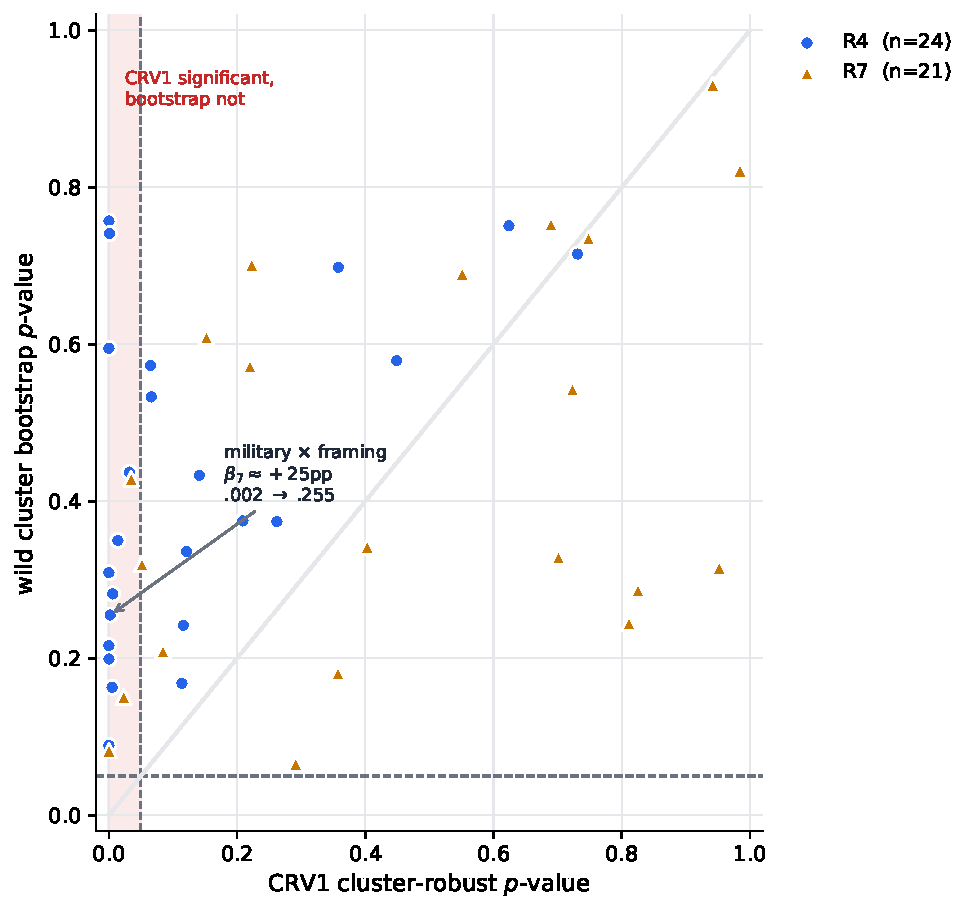
\includegraphics[width=0.78\linewidth]{figures/r4r7_crv1_vs_wcb.pdf}
  \caption{The CRV1-to-bootstrap collapse across both causal designs. Each point
  is one difference-in-differences estimate from R4 (per-event $\beta_3$ and
  crisis-type $\beta_7$) or R7 (per-event and pooled $\beta_3$); axes are its
  cluster-robust (CRV1) and wild-cluster-bootstrap $p$-values. Of 45 estimates,
  15 are CRV1-significant and \emph{none} survive the bootstrap: every point in
  the shaded CRV1-significant column sits above the $0.05$ line, and no point
  falls below the diagonal. The headline candidate --- military crises moving
  stake-holding communities toward security-and-military framing by
  $\beta_7\approx+25$pp --- moves from $p=0.002$ to $0.255$. \textbf{The catch to
  read off this figure: the two inference methods disagree systematically in one
  direction, so on a panel of this shape a CRV1 $p$-value is not trustworthy on
  its own.}}
  \label{fig:crv1-wcb}
\end{figure}


%% ===========================================================================
\section{Figure plan}


%% Example figure stub -- uncomment and point at a real file once figures are
%% copied into the Overleaf project.
%%
%% \begin{figure}[h]
%%   \centering
%%   \includegraphics[width=\linewidth]{r5_ame_plot}
%%   \caption{Average marginal effects on P(Negative) and P(Positive) by frame
%%     and community, with King-Tomz-Wittenberg simulation CIs.}
%%   \Description{TODO: plain-text description under 2000 characters.}
%%   \label{fig:ame}
%% \end{figure}
